\documentclass[a5paper]{article}
\usepackage[utf8]{inputenc}
\usepackage[T1]{fontenc}
\usepackage{txfonts}
\usepackage{bm}
\usepackage{geometry}
\usepackage{graphics}

\title{Trigonometry}
\author{Jon Hurst}

\begin{document}
\maketitle
\section{Unit circle}

\begin{figure}[ht]
  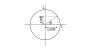
\includegraphics{trig-unit-circle}
  \caption{sin and cos on the unit circle}
   \label{fig:1}
\end{figure}

From Figure \ref{fig:1}, $\sin(\theta)$ is the projection of the line on the
y-axis and $\cos(\theta)$ is the projection on the x-axis. The gradient of the
line is equal to $\tan(\theta)$.

Since $x^2 + y^2 = 1$ for a unit circle

\begin{equation} \label{eq:4}
  \cos^2(\theta) + \sin^2(\theta) = 1
\end{equation}

Dividing (\ref{eq:4}) through by $\sin^2(\theta)$ and $\cos^2(\theta)$
respectively gives

\begin{eqnarray}
  1 + \tan^2(\theta)  & = & \sec^2(\theta)\\
  \cot^2(\theta) + 1 & = & \csc^2(\theta)
\end{eqnarray}

It can also be seen from Figure \ref{fig:1} that $\sin(\theta)$ and
$\cos(\theta)$ are periodic with period $2\pi$, whereas $\tan(\theta)$, being
the gradient of the line, is periodic with period $\pi$.

\begin{figure}[h]
  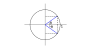
\includegraphics{trig-unit-circle-negative-theta}
  \caption{Negative $\theta$ relationships}
   \label{fig:2}
\end{figure}

\vbox{
Figure \ref{fig:2} illustrates the following relationships:
\begin{eqnarray}
\cos(\theta)&=&\cos(-\theta)\\
\sin(\theta)&=&-\sin(-\theta)\\
\tan(\theta)&=& -\tan(-\theta)
\end{eqnarray}
}

\begin{figure}[h]
  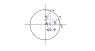
\includegraphics{trig-unit-circle-90}
  \caption{Co relationships}
   \label{fig:4}
\end{figure}

Figure \ref{fig:4} illustrates the following relationships, which are
essentially the definition of the ``co'' part of the trig names

\begin{eqnarray}
  \cos(\theta)&=&\sin(\frac{\pi}{2} - \theta)\\
  \sin(\theta)&=&\cos(\frac{\pi}{2} - \theta)
\end{eqnarray}

\vbox{
  From these, the rest of the ``co'' relationships can be derived:

\begin{eqnarray}
  \sec(\theta)&=&\csc(\frac{\pi}{2} - \theta)\\
  \csc(\theta)&=&\sec(\frac{\pi}{2} - \theta)\\
  \tan(\theta)&=&\cot(\frac{\pi}{2} - \theta)\\
  \cot(\theta)&=&\tan(\frac{\pi}{2} - \theta)
\end{eqnarray}}

\begin{figure}[h]
  \includegraphics{trig-unit-circle-180}
  \caption{$\pi$ relationships}
   \label{fig:5}
\end{figure}

Figure \ref{fig:5} illustrates the following relationships:

\begin{eqnarray}
  \cos(\theta) & = & -\cos(\pi - \theta) \\
  \sin(\theta) & = & \sin(\pi - \theta) \\
  \tan(\theta) & = & -\tan(\pi - \theta)
\end{eqnarray}


\section{Multiple angle identities}

\begin{figure}[ht]
  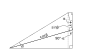
\includegraphics{trig-multiple-angle}
  \caption{Multiple angle for sin}
   \label{fig:3}
\end{figure}

\vbox{From figure \ref{fig:3} we derive the following basic formulae:

\begin{eqnarray}
  \sin(\alpha + \beta) & = & \sin(\alpha)\cos(\beta) + \cos(\alpha)\sin(\beta) \label{eq:5}\\
  \sin(\alpha - \beta) & = & \sin(\alpha)\cos(\beta) - \cos(\alpha)\sin(\beta) \label{eq:6}
\end{eqnarray}}

Replacing $\alpha$ by $\frac{\pi}{2} - \alpha$ gives

\begin{eqnarray}
  \cos(\alpha + \beta) = \cos(\alpha) \cos(\beta) - \sin(\alpha) \sin(\beta) \label{eq:7}\\
  \cos(\alpha - \beta) = \cos(\alpha) \cos(\beta) + \sin(\alpha) \sin(\beta) \label{eq:8}
\end{eqnarray}

Combining (\ref{eq:5}) with (\ref{eq:7}) and (\ref{eq:6}) with (\ref{eq:8}) gives

\begin{eqnarray}
  \tan(\alpha + \beta) & = & \frac{\tan(\alpha) + \tan(\beta)}{1 - \tan(\alpha)
    \tan(\beta)} \label{eq:9}\\
  \tan(\alpha - \beta) & = & \frac{\tan(\alpha) - \tan(\beta)}{1 + \tan(\alpha) \tan(\beta)}
\end{eqnarray}

Equations (\ref{eq:5}) to (\ref{eq:8}) can also be added or subtracted to
produce identities for expressions such as $2\sin(\alpha)\cos(\beta)$.

Setting $\beta = \alpha$ in (\ref{eq:5}), (\ref{eq:7}) and (\ref{eq:9}) gives
the double angle formulae

\begin{eqnarray}
  \sin(2\alpha) & = & 2 \sin(\alpha) \cos(\alpha) \\
  \cos(2\alpha) & = & \cos^2(\alpha) + \sin^2(\alpha) \label{eq:1}\\
  \tan(2\alpha) & = & \frac{2 \tan(\alpha)}{1 - \tan^2(\alpha)}
\end{eqnarray}

Substituting (\ref{eq:4}) gives alternate forms of (\ref{eq:1})

\begin{eqnarray}
  \cos(2\alpha) = 2 \cos^2(\alpha) - 1 \label{eq:2}\\
  \cos(2\alpha) = 1 - 2 \sin^2(\alpha) \label{eq:3}
\end{eqnarray}

Rearranging (\ref{eq:2}) and (\ref{eq:3}) gives

\begin{eqnarray}
  \cos^2(\alpha) = \frac{1}{2}(1 + \cos(2\alpha)) \\
  \sin^2(\alpha) = \frac{1}{2}(1 - \cos(2\alpha))
\end{eqnarray}
\end{document}
